%!TEX root = ../main.tex
\chapter{结合标签主题的跨域推荐算法}

\section{初步定义}
假定,我们有用户的集合 $\mathbb{U}=\{u_1,\dots,u_I \}$,这些用户用一组标签 $\mathbb{T}=\{t_1,\dots,t_N \}$ 标记了的一组物品 $\mathbb{V}=\{v_1,\dots,v_J \}$,以及评分的集合  $\mathbb{R}=\{R_1,\dots,R_O \}$,其中,$I$ 、$J$、$N$ 和 $O$ 依次代表了用户、物品、标签和评分的数目。每一个用户-物品-标签-评分(U-I-T-R)的可见数据是一个四元组 $(u, v, T_{ij}, R_{ij})$,其中 $u \in \mathbb{U}$,$v \in \mathbb{V}$,$T_{ij} \subset \mathbb{T}$ 是用户 $u$ 赋予物品 $v$ 的标签集合 ,$R_{ij}$ 是用户 $u$ 对物品 $v$ 的评分。

$P \in R^{f*I}$ 表示用户的潜在特征矩阵,其中列向量 $p_u$ 表示用户 $u$ 的 $f$ 维潜在特征向量。$Q \in R^{f*J}$ 表示物品的潜在特征矩阵,其中列向量 $q_v$ 表示物品 $v$ 的 $f$ 维潜在特征向量。$Y \in R^{f*N}$ 表示标签的潜在特征矩阵,其中列向量 $y_t$ 表示标签 $t$ 的 $f$ 维潜在特征向量。

对于基于标签和评分的推荐中,给定现有的四元组 U-I-T-R ,我们的目标是预测用户 $u_i$ 对物品 $v_j$ 的未知的评分。

\section{单一域建模}
我们首先在单一域上将标签信息引入矩阵分解,提出结合标签的协同过滤模型。直观上,用户给物品赋予的标签提供了物品评分的额外信息,因此我们认为引入标签会有助于评分预测的效果。

\subsection{低相关标签过滤}
现实系统中,用户会赋予物品大量的各种各样的标签,例如,一部电影被赋予的标签可能是主演的名字、上映年份,也可能是只有某个用户自己理解的标注(比如该用户观看影片时的天气),因此不同的标签与评分具有不同的相关性。实际上,互联网上的很多数据都大致服从一种称为 PowerLaw 的分布,该分布说明标签的流行度 $k$ 与流行度为 $k$ 的标签总数成反比。图\ref{fig:powerlaw} 显示了 MovieLens 和 LibraryThings 数据集的标签流行度的长尾分布,它们的双对数曲线几乎是一条直线。
\begin{figure}[htbp]
\centering
\subfigure[MovieLens]{
\label{fig:powerlaw:movielens}
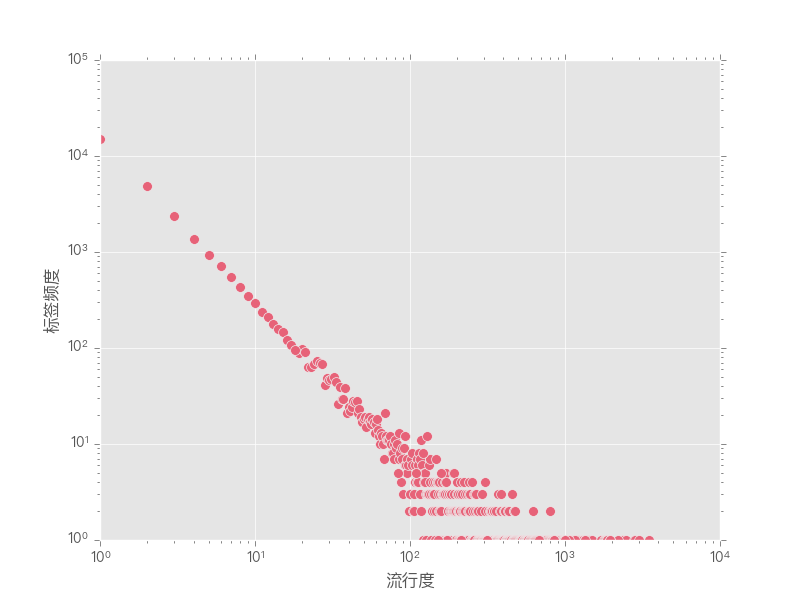
\includegraphics[width=0.48\linewidth]{images/powerlaw1.png}
}
\subfigure[LibraryThings]{
\label{fig:powerlaw:librarythings}
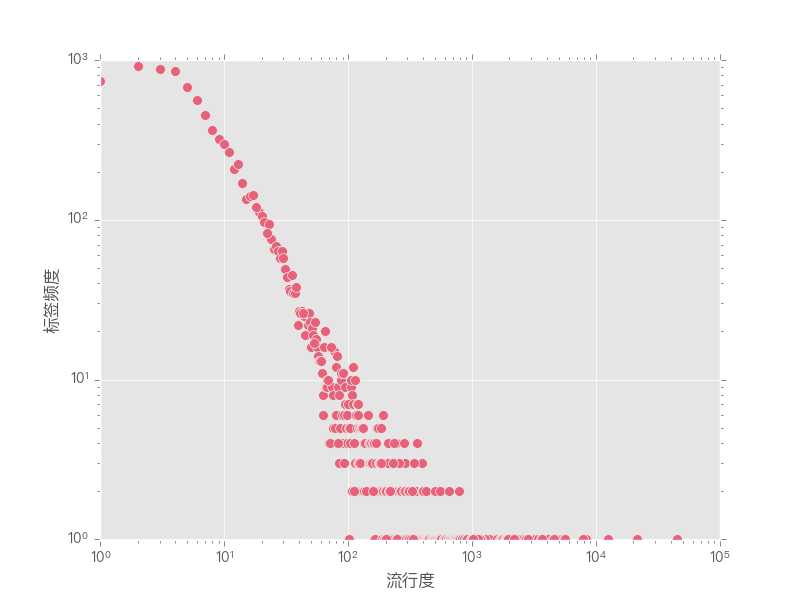
\includegraphics[width=0.48\linewidth]{images/powerlaw2.png}
}
\caption{标签流行度的长尾分布。横坐标是流行度 $k$ ,纵坐标是数据集中流行度为 $k$ 的标签总数 $n(k)$ 。}
\label{fig:powerlaw}
\end{figure}
从图中看出,大部分标签出现的频率都很低,只有很少的标签被经常使用。所以我们只考虑那些对评分预测具有帮助的标签,减小不相关标签引入的噪声。为了评估一个标签与评分是否相关,需要比较在该标签出现和不出现两种情况下的评分样本分布。我们使用 Wilcoxon 秩和检验,设置 $95\%$ 置信度,因此,当具有某个标签的评分与不具有该标签的评分之间具有显著差异时,我们认为该标签与评分是相关的。

\subsection{结合物品标签的协同过滤}
为了解决 UserItemTags 模型在预测时需要目标标签的限制,我们考虑任何用户赋予目标物品的全部相关标签集合 $TR(i)$ ,因为物品被赋予的任何相关标签都可能影响该物品的评分。如果一个标签被多次赋予一个物品,那我们认为这个标签更好的反映了该物品的特性,因此在模型中引入标签的出现频率,提升高频标签对评分的影响。我们用 $TRo_i$ 表示物品 $i$ 的全部相关标签数目(计入重复出现的标签),用 $TRo_i(t)$ 表示标签 $t$ 在物品 $i$ 上出现的次数。首先提出结合物品标签的协同过滤模型(collaborative filtering with item tags, 简称 ITCF),将物品标签信息融入预测模型中,对于给定用户 $u$ 和物品 $i$ ,按如下方式预测评分:
\begin{equation}
\hat{r_{ui}} =  \mu + b_i + b_u  +  p_u^T \cdot (q_i + \frac{1}{|TRo_i|}  \sum\limits_{t  \in TR(i)} {TRo_i(t) y_t}  ),
\end{equation}
其中,$p_u$,$q_i$ 和 $y_t$ 分别是用户 $u$、物品 $i$ 和标签 $t$ 的潜在特征向量。$\mu$ 是全部评分的平均值, $b_u$ 和 $b_i$ 是在用户 $u$ 和物品 $i$ 的偏移量(为了简明的描述我们的模型,之后的公式中不再显示地写出偏移项,而默认都是存在偏移项的)。模型参数的学习方法与传统的矩阵分解模型相同,采用随机梯度下降最小化正则平方误差:
\begin{equation}
\min_{q^*, p^*} {
\sum\limits_{u,i} {(r_{u,i} -  p_u \cdot (q_i + \frac{1}{|TRo_i|}\sum\limits_{t \in TR(i)}{TRo_i(t) y_t}))^2}
+ \lambda( \sum\limits_{u} ||p_u||^2+ \sum\limits_{i} ||q_i||^2 + \sum\limits_{t} ||y_t||^2 )}.
\end{equation}


遍历所有已知评分项(U-I-T-R),参数迭代方式如下:
\begin{equation}
\begin{aligned}
&-q_i \leftarrow q_i + \gamma \cdot(e_{ui} \cdot p_u -\lambda \cdot q_i)     \\
&-p_u \leftarrow p_u + \gamma \cdot(e_{ui} \cdot (q_i + \frac{1}{|TRo_i|}  \sum\limits_{t  \in TR(i)} {TRo_i(t) y_t})- \lambda \cdot p_u)    \\
&-\forall t \in TR(i) : y_t \leftarrow y_t + \gamma \cdot(e_{ui} \cdot p_u \cdot \frac{1}{|TRo_i|} \cdot TRo_i(t)  -\lambda \cdot y_t)     \\
\end{aligned}
\end{equation}

需要注意的是,在遍历已知项进行参数迭代时,对于每一个评分项都要对该物品所有的标签进行遍历。实际的数据集中,物品被标注的标签数目往往是巨大的,因此考虑到计算的时间复杂性,该模型是不那么可行的。

\subsection{标签主题聚类}

上面的模型中,我们将标签表示为低维的特征向量的形式,使物品标签信息融入了矩阵分解模型,然而该模型的问题是计算复杂度比较大。因此,我们对物品所关联的标签集 $TR(i)$ 进行聚类,去除冗余信息的同时扩充标签的含义,例如,“个性化”和“协同过滤”含义相似,可以将它们划分为同一类别考虑。将每个物品被赋予的标签集合看作“文档”,所有物品的标签集组成了文档集。由于标签是无序的,我们使用 LDA 主题模型进行文档分类, LDA 是典型的词袋模型,它不考虑文法以及词的顺序。

不同于其他聚类模型限定一篇文档只能属于一个类别,LDA 展示了文档在多个主题上表现出的相关性。LDA 从大量文档集合中发现一组主题 $\beta_{1:K}$,其中主题是关于词项的分布,这些主题通常是直观的可解释的。同时得到每篇文档的主题分布 $\theta_{1:J}$ ,将物品的标签集 $TR(i)$ 在 $K$ 个主题上的情况刻画出来,提供了物品标签集 $TR(i)$ 的低维表示。主题的词分布和文档的主题分布都是多项式分布。

为了结合协同过滤和主题模型,将物品的标签主题分布向量 $\theta_i$ 与之前矩阵分解中的物品特征向量 $q_i$ 结合起来,以它们的和作为物品的特征,从而评分预测为:
\begin{equation}
\hat{r_{ui}} =  p_u \cdot (q_i + \theta_i).
\end{equation}
因此,一个物品的标签主题分布揭示了该物品的特性,而一个用户特征向量每个维度上的数值表示了该用户对每个主题的偏好程度,这使得潜在特征向量是可解释的。在该模型中,标签主题的数目 $K$ 被限制与潜在特征的因子数相同,通常情况下,特征向量的维数 $f$ 在 20 到 200 之间\cite{Koren2009Matrix}。为了能更灵活地调整标签的主题分布情况,我们改变该模型的形式,为每个主题 $j$ 定义 $f$ 维特征向量 $z_j$ ,$Z \in R^{f*K}$ 表示主题的特征矩阵。将物品特征向量 $q_i$ 与加权平均的主题特征向量的和作为物品的特征表示,提出结合标签主题的协同过滤模型(collaborative filtering with tags topic,简称 TTCF),该模型以如下方式预测评分:
\begin{equation}
\label{TTCF}
\hat{r_{ui}} =   p_u^T \cdot (q_i +   \sum\limits_{j =1}^K {  {\theta_i}_j   z_j}  ),
\end{equation}
其中,主题特征的权值 ${\theta_i}_j $ 是主题分布 $\theta_i$ 在主题 $\beta_j$ 上的概率值,因为主题分布 $\theta_j$ 是多项式分布,所以权值的加和为 1,省去了计算加权平均时的分母部分。通过随机梯度下降最小化正则均方误差来学习模型的参数:
\begin{equation}
\begin{aligned}
&-q_i \leftarrow q_i + \gamma \cdot(e_{ui} \cdot p_u -\lambda \cdot q_i)     \\
&-p_u \leftarrow p_u + \gamma \cdot(e_{ui} \cdot (q_i +  \sum\limits_{j =1}^K {  {\theta_i}_j   z_j}  )- \lambda \cdot p_u)    \\
&-Z \leftarrow Z + \gamma \cdot(e_{ui} \cdot p_u \cdot  \theta_i^T -\lambda \cdot Z)     \\
\end{aligned}
\end{equation}

我们利用主题建模去除了标签的冗余,使得模型在计算复杂性方面变得可行,同时,主题建模对标签的含义进行了扩充,缓解了数据稀疏性问题。一个直观的好处是对于新物品的冷启动问题,可以从它的少量标签快速地获得主题,从而利用主题分布进行预测。


\section{跨域推荐模型}
在 3.2 中我们阐述了在单一域将标签信息引入矩阵分解的方法,利用主题建模缓解了数据稀疏性问题和冷启动问题。在本节中,我们引入跨域推荐的思想,将结合标签主题的协同过滤方法扩展到多个域上,利用辅助域的信息缓解目标域的数据稀疏性问题。

跨域推荐的关键挑战是在不同域的项目和用户之间发现有用的联系,通常所考虑的域之间看上去是不相关的,例如,音乐与感兴趣的地方,很难找到它们之间的关联。我们将标签作为连接不同域的桥梁,依赖于不同域中的重叠的标签词汇,例如,标签“romantic”可以用于描述一个电影,也可以是一首歌曲或是一处风景,换句话说,我们推测标签的影响是跨域的。因此,目标域可以学习到辅助域中的某个标签对评分的影响,即,如果在辅助域中的某个标签存在时,关联的评分通常较高,则可以将这种依赖关系从辅助域传递到目标域。将上面的预测模型$\eqref{TTCF}$ 扩展到多个域,对于每一个域 $d$ ,该推荐域中的评分预测模型为:
\begin{equation}
\hat{{r_d}_{ui}} = {p_d}_u^T \cdot ({q_d}_i +   \sum\limits_{j =1}^K {  {{\theta_d}_i}_j   z_j}  ),
\end{equation}
其中,${p_d}_u$ 和 ${q_d}_i$ 分别是推荐域 $d$ 所属的的用户和物品的潜在特征向量,${\theta_d}_i$ 是推荐域 $d$ 中的物品 $i$ 的标签主题分布。而主题的特征矩阵 $Z$ 则在多个域间共享,这样就通过标签主题在多个域间实现了相互影响。在参数学习中遍历两个域的可见项,利用随机梯度下降最小化正则均方误差。

\section{本章小结}
本章中,我们首先对基于标签的推荐问题进行了定义,然后提出了单个域上结合物品标签的协同过滤模型 ITCF,并指出了该模型在时间复杂性上的缺陷。继而提出结合标签主题的模型 TTCF,利用主题建模去除标签的冗余,并对标签的含义进行扩充,缓解了单个域上的物品冷启动问题和数据稀疏性问题。最后我们引入跨域推荐的思想,将单个域的模型扩展到多个域上,使得多个域的标签信息可以同时被利用来促进各个域上的预测效果。


